\documentclass[conference]{IEEEtran}
\IEEEoverridecommandlockouts
% The preceding line is only needed to identify funding in the first footnote. If that is unneeded, please comment it out.
\usepackage{cite}
\usepackage{amsmath,amssymb,amsfonts}
\usepackage{algorithmic}
\usepackage{graphicx}
\usepackage{textcomp}
\usepackage{float}

\def\BibTeX{{\rm B\kern-.05em{\sc i\kern-.025em b}\kern-.08em
    T\kern-.1667em\lower.7ex\hbox{E}\kern-.125emX}}
\begin{document}

\title{Paper Title\\}

\author{\IEEEauthorblockN{Andrii Fedorenko}
\IEEEauthorblockA{\textit{University of Vienna} \\
Vienna, Austria \\
andriifedorenko@gmail.com}
\and
\IEEEauthorblockN{Aliaksandr Adamenko}
\IEEEauthorblockA{\textit{University of Vienna} \\
Vienna, Austria \\
alexadamenko@gmail.com}
\and
\IEEEauthorblockN{Erich Schikuta}
\IEEEauthorblockA{\textit{University of Vienna} \\
Vienna, Austria \\
erich.schikuta@univie.ac.at}
}

\maketitle

\begin{abstract}
 TODO
\end{abstract}

\begin{IEEEkeywords}
TODO
\end{IEEEkeywords}

\section{Introduction}
TODO

\section{Related Work and Baseline Research}
TODO

\section{System Architecure (!!!! RENAME)}
\subsection{Competitors (!!!RENAME)}
TODO

\section{Contemporary User Interface}

The user-centered design is a fundamental requirement for N2Sky. Looking back on past experiences with the application, there were identified the real capabilities and needs of a users. N2Sky was moved from a complex expert system to an easy understandable application. Every interested user without having a deep knowledge in the neural network field can freely use N2Sky.  The goal was to save and gain the current functionality of the application and decrease the visual complexity of it. 

\subsection{Frontend and services}

N2Sky today is the cross-platform handy application with a responsive design. The frontend is written on ReactJS framework and it is convertible to the React-Native framework. The application is accessible from desktop computers, as well as from mobile devices or  other devices with any operational system. Furthermore, backend has microservices architecture to support scalability. Each one of the microservices is developed on NodeJS server, which implies efficiency and lightweight. This architecture enables its users to freely and easily work with the application without interruptions or waiting until it is completely loaded. 


\subsection{Modular design}

The central concept of the application is to support the Software as a Service (SaaS) and Platform as a Service (PaaS) distributions.  N2Sky consist of two modules: administration module, main application module.

\paragraph{Administration module} The administration module allows the system administrator to control the environment. The module supports OpenStack and Cloudify monitoring. Managing is possible through the application dashboard. It also contains custom monitoring and an alerting management system, which can be installed on any server within the N2Sky user interface. The administration module implements PaaS. It is fully configurable and wrapped into the open source project in order to make the module accessible to the third-party applications. 
\paragraph{Main application module} The main application module is the central module of N2Sky. Within this module, users can use, train and test existing neural networks. It is possible to reuse the neural network paradigms and create own neural network. N2Sky allows to deploy own network and store data in cloud. Module services are supporting the SaaS distribution. Experts can use an application directly through the N2Sky API or they can integrate N2Sky services to their own application. 

\subsection{User roles}

In order to make the N2Sky user interface understandable for arbitrary users as well as professional for advances users, it was decided to separate the user roles. Every user role has own way of interaction with the application:
\begin{itemize}
\item The contributor is an arbitrary user. Such a user has no necessity in having deep knowledge of the neural network field or know any programming language. The main goal of arbitrary user is to study neural networks within N2Sky. The contributor has an access only to his own dashboard and public available resources on the main application module. He can perform semantic search for available neural network paradigms and use them. He can also train running neural network instances and test them. This user can share his trained neural network by making it public. 
\item The developer is an expert user, which has enough knowledge and experience to create his own neural network. This user can create neural network paradigms using the ViNNSL schema and publish them on N2Sky. This user can deploy neural networks on the N2Sky environment as well as on his own environment by providing training and testing endpoints. The goal of the developer is the study how his networks will behave with different network structures, input parameters and training data that is provided by other users.
\item System administrator is a user who has a full access to application including environment management, monitoring and alerting features. Administrator can manage Openstack and Cloudify instances. He also can shadow any N2Sky user to observe the application from shadowed user perspective. Administrator has access to all dashboards in every module.
\end{itemize}


\section{Use Cases}

Workflow of solving problems as a contributor or a developer differs. If contributor needs an easy step-by-step workflow, the developer just wants to perform procedure quickly without any additional destructions. There are only a few pre-requirements, which will remain the same: authentification within N2Sky and the creation of a first project from the N2Sky dashboard, which describes the problem field.

\subsection{Creation of the new project by contributor}

After creating the project user has few possibilities to find a neural network, which corresponds his needs: create neural network from the paradigm or perform semantic search in order to find already available neural networks. 

\paragraph{Creating neural network from paradigm} User has to choose a paradigm and add it to his project. He has to fill out the network description form. The description form defined by ViNNSL schema. The mandatory fields are name, description, propagation type, learning type, application field and problem type. All this information will be user for semantic searching by other users. It is also necessary to define the network structure as it shown in ``Fig.~\ref{fig:structure}''. The structure definition can be absolutely customised. It is also possible to add a shortcut connection. The user does not have to have any concerns about correctness of the neural network structure. The application will take care of any errors and mistakes, which user can do. 


\begin{figure}[H]
  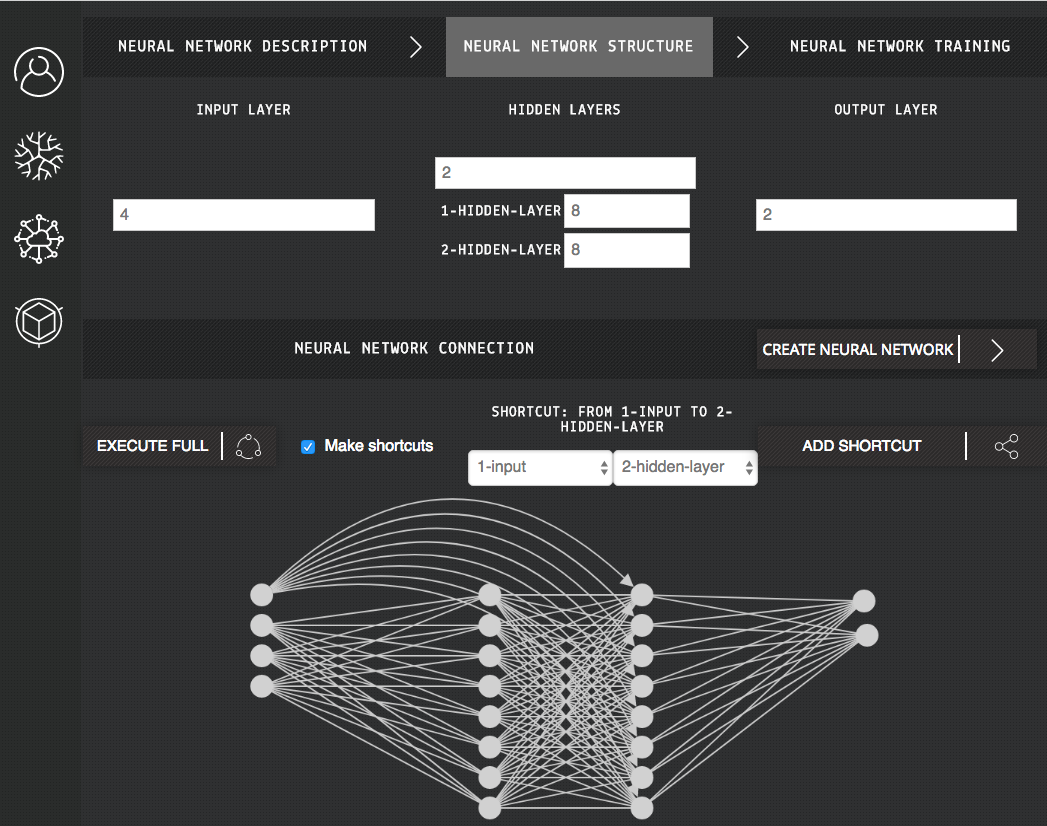
\includegraphics[width=\linewidth]{structure.png}
  \caption{Neural network structure definition}
  \label{fig:structure}
\end{figure}

After creating a neural network, the user will be redirected to the training view which is shown in ``Fig.~\ref{fig:training}''. From here he can run the neural network instance on N2Sky and publish it to make neural network available for the rest of the users. In case if user wants to study neural network in details he can also download it in ViNNSL format . Most importantly, the user can perform training. Since the neural network was created from the paradigm, default parameters for training are being set, which guide user in further steps.


\begin{figure}[H]
  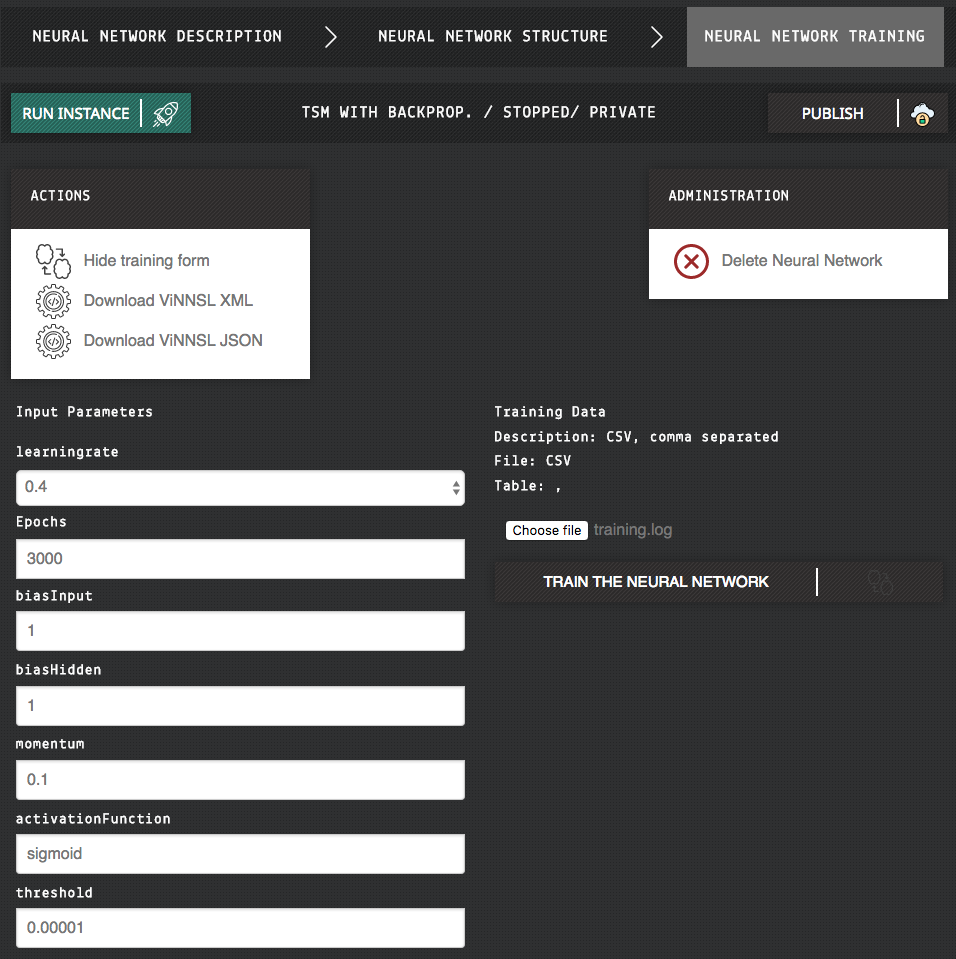
\includegraphics[width=\linewidth]{training.png}
  \caption{Neural network training view}
  \label{fig:training}
\end{figure}

The training form in  ``Fig.~\ref{fig:training}'' shows input parameters, which are needed to perform training. Input parameters as well as requirements for training file are defined in ViNNSL schema. 
Neural network training could take a while, but the user will not be blocked. Contributor can observe every evaluation step. After training is completed, the user can perform testing``Fig.~\ref{fig:eval}''. There is visual representation of evaluation will be shown.  The learning curve represents is constantly updating during neural network training. The x-Axis shows epochs and the y-Axis shows costs. 

It is also possible to publish trained model so that other users could test it with their own data.


\begin{figure}[H]
  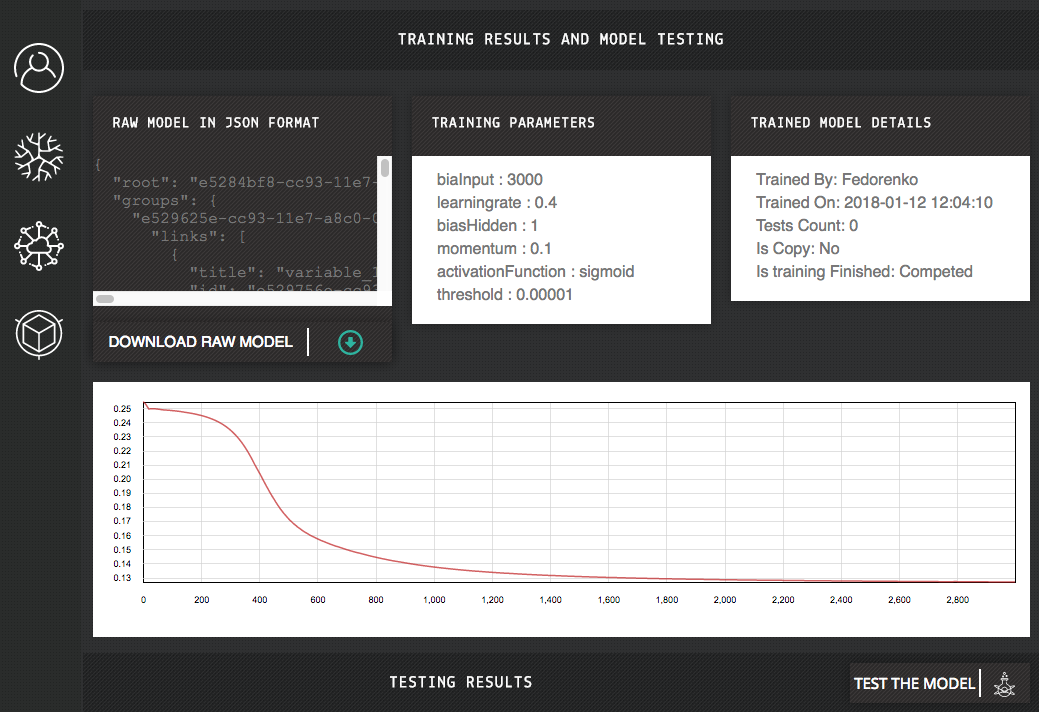
\includegraphics[width=\linewidth]{eval.png}
  \caption{Neural netowork evaluation process}
  \label{fig:eval}
\end{figure}

\subsection{Reusing existing neural network}

 N2Sky has neural network repository, which represents different solution for typical problems. The user can reuse already it.. The user has to navigate to neural network repository view as shown in ``Fig.~\ref{fig:repo}''  and copy the needed neural network to his own project. Start indicator represents copying functionality. If star is grey, than user can copy it to his project.  The user can perform training and testing on the copied networks. 

\begin{figure}[H]
  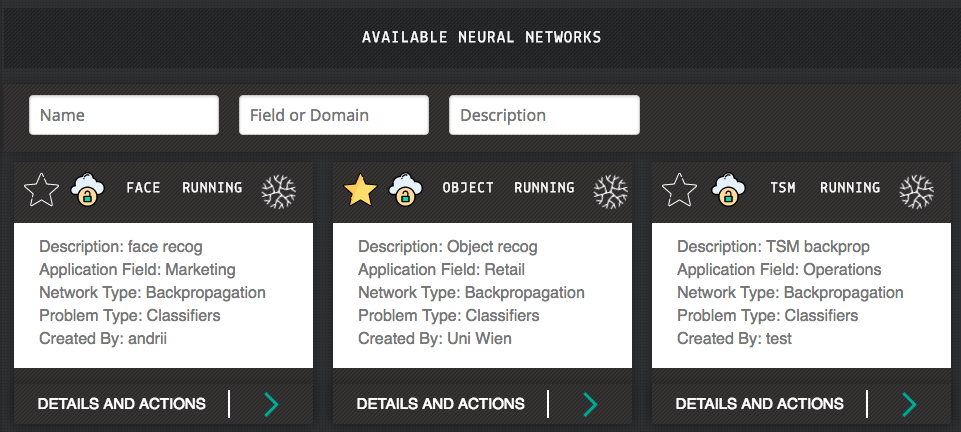
\includegraphics[width=\linewidth]{repo.png}
  \caption{N2Sky neural network repository}
  \label{fig:repo}
\end{figure}


\subsection{Creation of the new project by developer}
The developer is an expert user. He can download the ViNNSL schema template from N2Sky, fill it up and customise his neural networks as he wishes as it shown in ``Fig.~\ref{fig:own}''. After creating a project, the user can just upload his ViNNSL formatted paradigm and deploy. If user want to deploy his network on N2Sky environment, he has to provide Docker image of his neural network in order. 

The expert user get additional functionality. He can deploy his neural network on own environment in order to see how his system will behave with a increasing traffic. The developer will receive training and testing information from other users, which were working with his neural network.

\begin{figure}[H]
  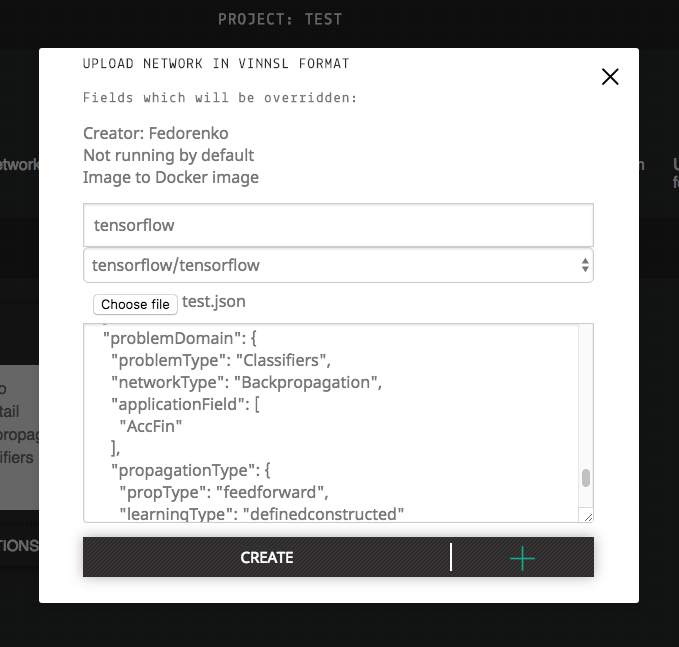
\includegraphics[width=\linewidth]{own_nn.png}
  \caption{Deploying own neural network on N2Sky}
  \label{fig:own}
\end{figure}

\section*{Acknowledgment}


\begin{thebibliography}{00}
\bibitem{b1} TODO
\end{thebibliography}

\end{document}
